\documentclass[12pt]{scrreprt}
\usepackage{listings}
\usepackage{underscore}
\usepackage{minted}
\usepackage[bookmarks=true]{hyperref}
\usepackage[utf8]{inputenc}
\usepackage[english]{babel}

\usepackage{tcolorbox}
\usepackage{hyperref}
\usepackage{amsfonts}
\usepackage{amsmath}
\usepackage{amssymb}

% \renewcommand{\cleardoublepage}{}
% \renewcommand{\clearpage}{}


% remember to document journey for the project also including challenges and what you did in project and other interesting stuff, not just reading off the report


\DeclareMathOperator*{\argmax}{argmax} % thin space, limits underneath in displays

\newcommand{\pr}{\mathbb{P}}

\hypersetup{
    bookmarks=false,    % show bookmarks bar?
    pdftitle={FP PROJECT REPORT},    % title
    pdfauthor={Saptarishi Dhanuka},                     % author
    pdfsubject={TeX and LaTeX},                        % subject of the document
    pdfkeywords={TeX, LaTeX, graphics, images}, % list of keywords
    colorlinks=true,       % false: boxed links; true: colored links
    linkcolor=blue,       % color of internal links
    citecolor=black,       % color of links to bibliography
    filecolor=black,        % color of file links
    urlcolor=purple,        % color of external links
    linktoc=page            % only page is linked
}%
\def\myversion{1.0 }
\date{}
%\title
\usepackage{hyperref}
\newcommand{\ttt}[1]{\texttt{#1}}


\begin{document}




% ·        Title (with name, ID, supervisor, date)

% ·        Acknowledgement, if any

% ·        Table of Contents

% ·        Introduction

% ·        Background and Motivation

% ·        Literature Survey (state-of-the-art) – Gap Analysis, Research Questions etc.

% ·        Problem Statement / Objectives

% ·        Scope, Methodology, and Design – Architecture, HLD / LLD, if applicable

%  can have naive bayes in the methodology

% ·        Work Done – Implementations, Challenges, Mitigations, etc.

% ·        Results and Discussions

% ·        Conclusions (should highlight contribution)

% ·        Extensions and Future Work

% ·        References

 

% NOTES
% midterm feedback: First the specs should just contain the input output and not the method
% Req
% Spec
% Analysis
% Then architecture and design

% Explore llm for identifying interesting

% Explore pldi type thing

% First the project assumes html on the basis of tags. If not based on tags the
% the thing breaks. The specs shouldnt mention tagsoup and stuff. Should be independent of the method. But it should mention the limitations (?)

% In specs reduce the scope to assuming that using html and the tags are there using the parenthesisation problem. No don't do that in specs do that in the design  

% Original requirement doesn't mention that tags are there

% Just web page and get code and text

% Can u identify the code and the text without knowing the tags

% Mention in analysis

% Design shouldnt have the function details and stuff

% Architecture and design comes after analysing the the specs and requirements

% Specs in the presentation are wrong

% Get feedback from prof about what to do in report



% The specs are wrong. The specs should firstly mention the input output again after the requirments and mention it more technically like what separates the code from the text. It should NOT mention tagsoup or anything related to the method


% In the analysis of the specs then we can say that one way to tackle this problem is by assuming that the given web page is formatted in an correct HTML structure. Then we can extract the tags and solve the parenthesization problem for getting the code and the text out





% design flows from the specs so shouldn't have the function details and stuff directly 


\begin{flushright}
    \rule{16cm}{5pt}\vskip1cm
    \begin{bfseries}
        \Huge{Functional Programming \\ CS-IS-2010-1 \\ Final Project Report }\\
        \vspace{1.1cm}
        Topic: Haskell Scraper and Code-Text Separation\\
        \vspace{1.1cm}
        Name: Saptarishi Dhanuka\\
        \vspace{1.1cm}
        ID: 1020211525\\
        \vspace{1.1cm}
        Supervisor: Partha Pratim Das\\
        \vspace{1.1cm}
        Date: 13 May 2024\\
        \vspace{1.1cm}
        Ashoka University\\
    \end{bfseries}
\end{flushright}


\newpage 


\tableofcontents

\newpage

\chapter{Acknowledgements}

I would like to thank Professor Das for taking this Independent Study Module and giving us the incentive to work on a software project in an unfamilar yet elegant language. I would also like to thank my fellow students as well as the teaching volunteers Gautam and Adwaiya for creating a wholesome learning environment. 


\chapter{Introduction}

%  cite stuff here cause references page is there and can't just say stuff in the air
%  maybe some motivation part here can go into the motivation section instead of the intro 

In the course, I worked on the scraper project to separate text and code snippets from a text source. After initially going down a highly restrictive path of HTML based classification, the feedback obtained from the midterm evaluation made me switch track and try to make a more general separator that would work on any text source and not just HTML formatted web pages. \\ I developed a Naive Bayes classifier for this problem since I looked at it from the lens of document classification, where each line in the given text source could be classified as being source code or text, and then finally all the lines of the same class would be separated into their respective files.\\ In terms of learning outcomes, I had started from being a complete novice in Haskell. The project enabled me to immerse myself in the sometimes frustrating but mostly elegant frameworks of the Haskell language and appreciate it's deep connect with formalisms. It also made me aware of the importance and relevance of the topic I was working on, as I shall elucidate further.\\
\\ The large amounts of data in the form of interspersed code and natural language make it useful to extract knowledge from them in order to benefit various areas of software development. Examples like natural language comments accompanying code, stackoverflow questions and answers with code blocks, and developer emails containing discussions about code with reference to it are all important forms of such data and contain valuable information that is waiting to be extracted. \\ 
\\ For instance, extracting code and natural language separately from developer emails at a company can give key insights about how the company codebase has evolved and can help future developers access the code of emails directly. Separation of code and natural language is also helpful as training data for natural language and code completion models which can used the separated text and code to give better results. It creates a structured view of the code and textual data which can then further be used to create an organized view of the code and associated natural language. The tool that I have made, albeit simplistic, can help towards extracting useful knowledge for software development in a lightweight manner. 


\chapter{Background and Motivation}


Consider the following image of an educational web page containing interspersed code and natural language:

\begin{figure}[h]
    \centering
    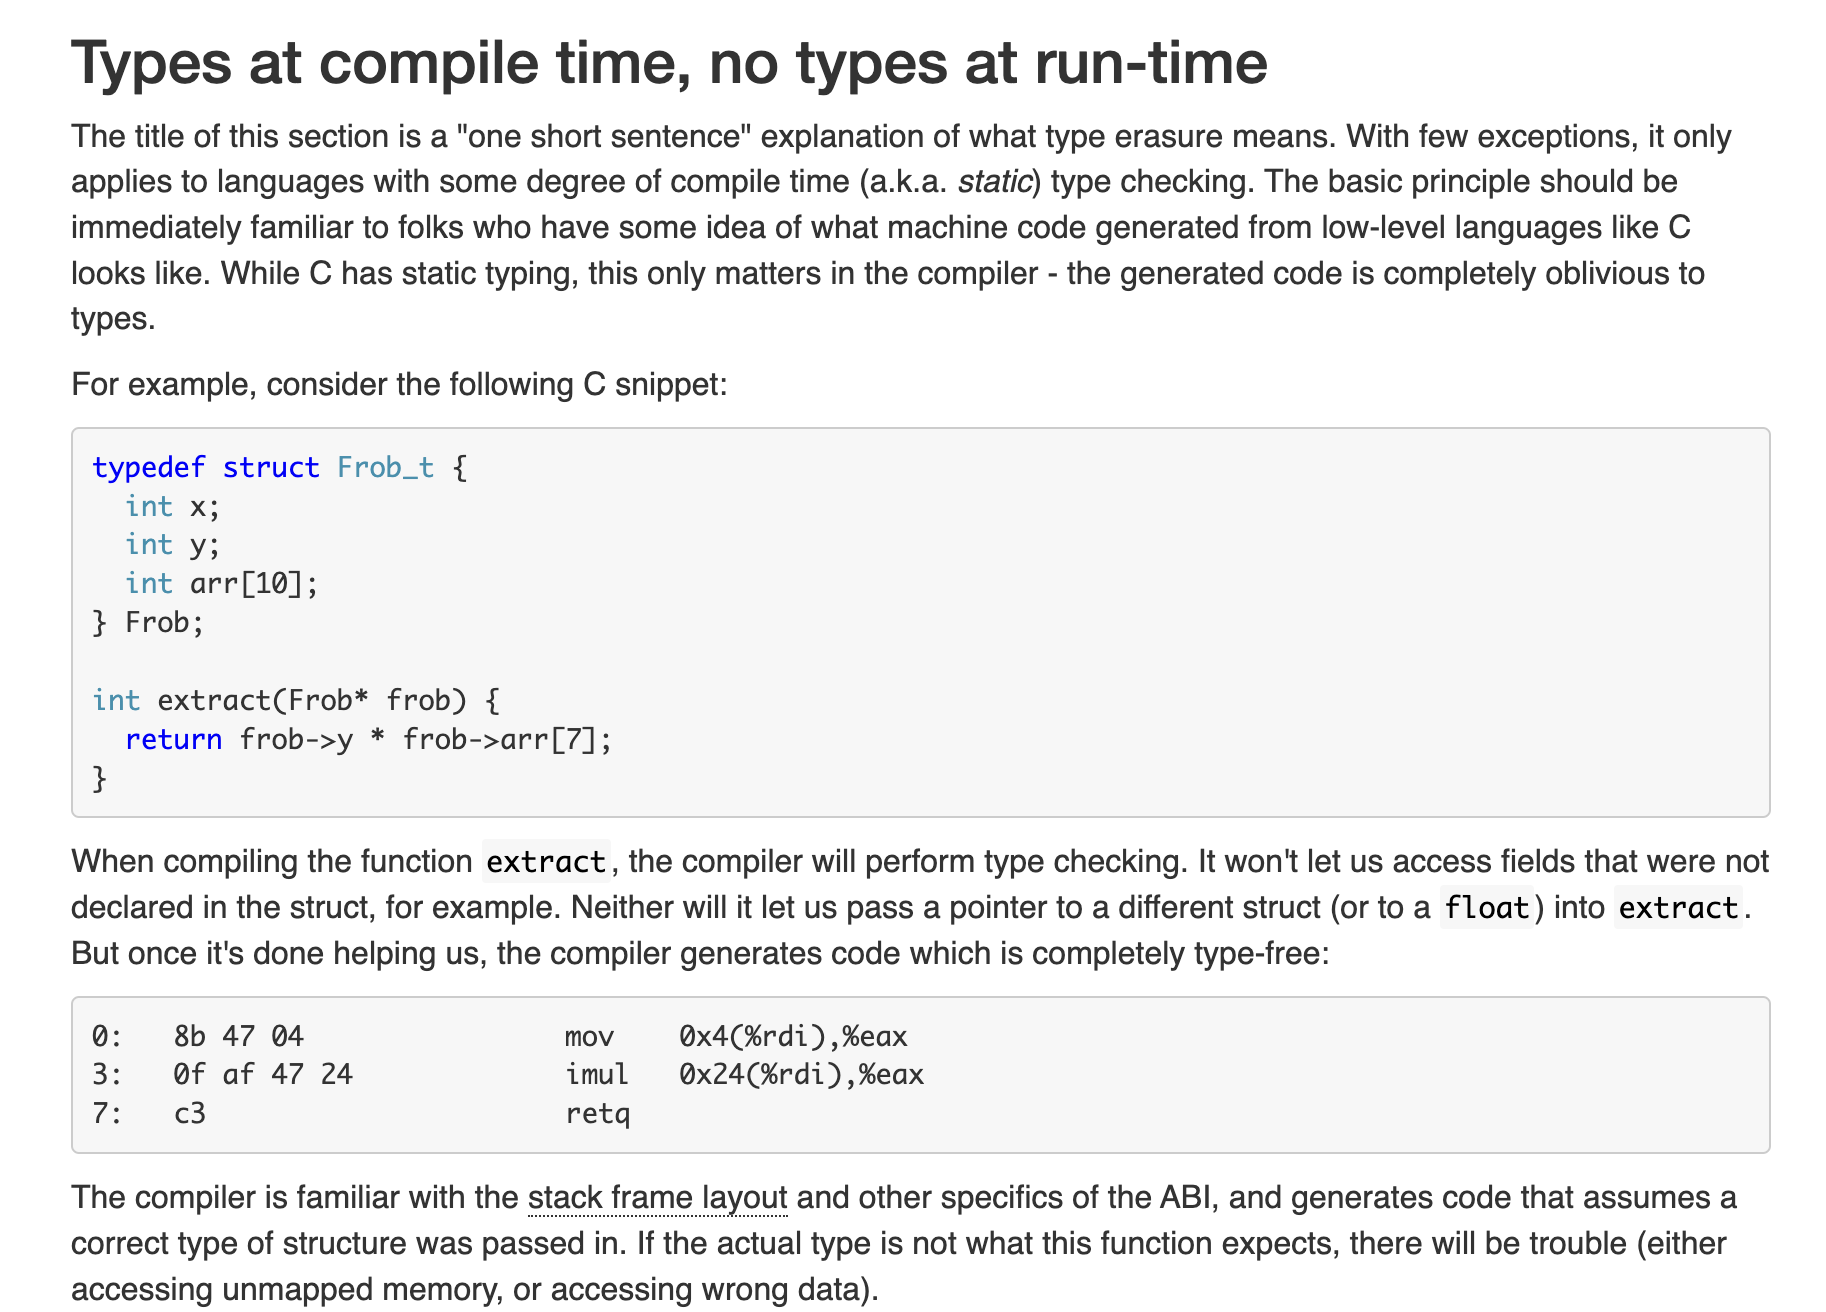
\includegraphics[width=0.7\textwidth]{figures/background-eg.png}
    \caption{Example of Code and Language Together}
    \label{fig:code-lang}
\end{figure}

Here it becomes useful to extract just the code or just the natural language separately if one just wants to run the code on their own machine or just wants the natural language descriptions for their notes or to get an overview of the idea being conveyed. \\ This is just one specific example where separating code and text yields valuable information extracted from a noisy text source. The project's domain extends to many other use cases as well. We already mentioned developer emails and stackoverflow Q \& A, but this information extraction can play an important role in just about any area where there is a large amount of code and natural language in one place, which further underlines the need for an efficient separator.


\chapter{Literature Survey}

%  maybe also see what all libraries and stuff for naive bayes and stuff are there in haskell rn

%  gap analysis and research questions ?????????????????

% basically that these guys did this and those guys did that and here's what I am gonna do and mention shortcomings and stuff later and say that did from scratch since haskell sde project
% should i mention the results of the literature here or when comparing with my own results in the results section??


\section{Research}


Researchers have used various methods to identify and distinguish code and natural language text, some of which I will discuss below. \\ Bacchelli et. al \cite{bachemail} attempted to extract source code from developer emails by first identifying emails that contained source code and then identifying code blocks by using regular expressions. The approach was very lightweight and programming language specific, with the use of end-of-line characters like semi-colons in order to find code lines. \\ Bacchelli et. al \cite{bachcontent} also used Naive Bayes with bigrams, in combination with island parsing for classifying pieces of development emails as various categories like code, natural language, stack trace, patch or junk. It reached an accuracy ranging between 89 and 94 \% but, the source code island parser was specific to Java, which the authors acknowledged and stated that the approach could be easily generalized to other languages too. \\ Chatterjee et. al \cite{chattter} focused on extracting the code segments along with their natural language descriptions from research articles using various detailed linguistic and structural heuristics to identify important features to identifying sentences that would be relevant to code segments. \\ Cerulo et. al \cite{cerulohmm} used an approach based on Hidden Markov Models (HMMs) for extracting "information islands" of code from natural language by recognising whether the sequence of observed strings would change between the source code and natural language states of the HMM. While this approach did not require parsing or complicated regular expressions, it only performed classification of tokens into code or text, and not further knowledge extraction in the form of an abstract syntax tree.\\ The Naive Bayes approach for text classification also has a long history and it is extensively used even today despite it's simplicity and strong assumptions \cite{juraf}, hence it is a promising candidate for this software project focused on learning Haskell.

\section{Library Support}

Before deciding to implement Naive Bayes from scratch, I attempted to look for lightweight libraries that could help me in separating code and text. First I tried the Hidden Markov Model library \href{https://hackage.haskell.org/package/hmm-0.1}{hmm}, I could not make to work properly. Searching for Naive Bayes in Haskell also led to very underdeveloped libraries such as \href{https://hackage.haskell.org/package/hext-0.1.0.4/docs/NLP-Hext-NaiveBayes.html}{NaiveBayes} or other individuals' projects that would not work efficiently with the task at hand. Not wanting to use other heavy ML methods, I decided to implement Naive Bayes from scratch in order to achieve maximum customisation and flexibility regarding my data and results.


\chapter{Problem Statement and Objectives}
\begin{tcolorbox}[colback=white,colframe=gray,title={Assigned Project Statement}]
    Develop a scraper using Haskell to extract text and code snippets separately.
    \begin{enumerate}
        \item \textbf{Input}: Scrape the text and code snippets from the given text source.
        \item \textbf{Output}: A Word document containing the text and \texttt{.txt} file containing the code.
        \item \textbf{Method}: Write the algorithm to scrape (you can use the \texttt{tagsoup} library) and all the input-output facilities using Haskell. Do not use any other language.
    \end{enumerate}
\end{tcolorbox}

% in the design section can give the basic structure of the HTML page

% \section{Problem Description}
% The given web page is made of text and code snippets, which we need to scrape and extract separately into a \texttt{.docx} file containing the text portions and a \texttt{.txt} file which has the code snippets. \\ For this, we need to fetch the given web page, parse and analyze it,so that we can effectively separate them into different documents.


\section{Requirements/Objectives}

\begin{enumerate}
    \item The user shall be able to give any text source as input.
    \item The scraper shall get all the code snippets of the source and write it into a Plaintext file.
    \item The scraper shall get all non-code text of the source and write it into a Word Document.
\end{enumerate}


\section{Specifications}

\begin{enumerate}
    \item The user will be able to enter a text source as input, whose code and non-code parts they wish to be separated.
    \item The scraper will parse the contents of the text and separate the code snippets from the rest of the text.
    \item The scraper will output a \texttt{.docx} file containing the textual content.
    \item The scraper will output a \ttt{.txt} file containing the code snippets.  
\end{enumerate}



% can mention that the scope is being restricted to with HTML stuff in the analysis
\section{Analysis}

\begin{enumerate}
    \item There are many ways of solving the problem both by syntactic and semantic approaches. Some semantic approaches are as follows:
        \begin{enumerate}
            \item Lexical and semantic analysis with the use of regular expressions
            \item Using a large language model to differentiate the code and the rest of the text 
            \item Using computer vision to attempt to read text like a human and identify text from the code
            \item Use the frequency of occurrence of different words in some sample data and use it to predict whether sections of unseen samples of text are natural language or source code. 
        \end{enumerate}
    \item Extracting the text and code snippets from a text source can boil down to a classification task where we consider each new line as a line to be classified as natural language or code, and grouping them all into two separate sections depending on the class assigned to them.
    \item Hence we restrict our project by considering that the text source will consist of different newlines which need to be classified as language or code, without going into further granular details as to whether a particular word or phrase is code or text. Our project will not consider that the text source will be devoid of newlines.
    %  we will take as input url but then just get the text from that url and nothing else. 
    

\end{enumerate}






\chapter{Scope and Methodology}

\section{Scope}
Following from the analysis, the system will classify text sources on a line level of granularity, hence it assumes that there will be some newline separation of different lines and the text source will not be completely unstructured. This is still a fairly broad scope since most text sources that have natural language and code interspersed in them have a newline-structure that make it easy to split them on a line-by-line basis for classification. Notwithstanding, we restrict our scope to exclude sources devoid of newlines since text and code separation in that case would need a more semantic approach that we will not consider.

% ADD STUFF HEREEEEEE!!!!

\section{Methodology}

The broad methodology is to train a Naive Bayes classifier on some custom training data consisting of natural language and source code, and then using the calculated probabilities to classify each line in the given text source as being code or natural language, and then separating them based on that. A brief overview of Naive Bayes is given below with the design and architecture covered later.
\subsection{Naive Bayes Overview}
Our main goal with Naive Bayes is to find, for each line in the text source, the best class (code or natural language) for it. That is, for each line $l$ made of some $t_k$ terms and class $c$, we want to find \\ $\hat{c}$ = $ \argmax_c \pr(c | l) = \argmax_c \pr(c | t_1, t_2, ... t_k)$. \\ Instead of just considering the terms occuring in the line, we will consider all words in the vocabulary from now and see if they are occuring in the line or not.\\
\\ First we consider the vocabulary of all the words in the training data. Now for each line in the text source, we have a binary feature vector whose elements are set to 1 if a word in the vocabulary occurs in that line, otherwise being set to 0. That is, if there are $n$ words in the vocabulary, then the feature vector $l_i$ corresponding to the $i$-th line will have $l_{ij} = 1$ if the $j$-th word from vocabulary occurs in the $i$-th line, otherwise being 0.\\
\\ Now we want to calculate $\mathbb{P}(l_i | y)$ where $y$ is a particular class like code or natural language. We make the strong Naive Bayes assumption that all the $l_{ij}$'s are conditionally independent given the class $y$. This is clearly not true in practice, but even with this assumption we get good performance. 
Moreover, we consider each line as an unordered Bag of Words where word position doesn't matter and only it's frequency matters, which is another strong assumption that the classifier operates under and performs surprisingly well.\\
\\ Hence $\mathbb{P}(l_{i1}...l_{in} | y)$ = $\prod_{j=1}^{n} \mathbb{P}(l_{ij} | y)$. \\
\\ Considering a particular line $l$ and using Bayes Rule we get:\\
\\  $\hat{c}$ = $ \argmax_c \pr(c | l) = \argmax_c ( \pr(l | c) \times \pr(c) )  = \argmax_c ( \pr(c) \times \prod_{j=1}^{n} \mathbb{P}(l_{j} | c) )$.\\
\\ Usually, the probability numbers computed are very small, so we work in the logspace by using the natural logarithm to avoid issues with numerical underflow.\\

$\therefore \hat{c} =  \argmax_c \log \pr(c | l) = \argmax_c \log( \pr(l | c) \times \pr(c)) = \argmax_c  \log (\pr(c) \times \prod_{j=1}^{n} \mathbb{P}(l_{j} | c) ) \\
\\ = \argmax_c (\log \pr(c) + \sum_{j=1}^{n} \pr(l_{j} | c)) $\\
\\ \textbf{How to calculate these terms?}\\
\\ We calculate $\pr(c)$ by just calculating what percentage of the training data belongs to that particular class. For each $\pr(l_j|c)$, we calculate the probability of the $j$-th word in the vocabulary being in the class $c$ by counting the number of times that word occurs in the class $c$ and dividing by the total number of words in the class $c$. Using a form of Laplace smoothing, we add small decimal numbers $\alpha$ and $\beta$ in the numerator and denominator to avoid 0 probability in case of completely unseen words for the unseen data.\\
\\ Hence $\pr(l_j|c) = \dfrac{count(l_j, c) + \alpha}{\beta + \sum_{j=1}^{n} count(l_j, c)}$ \\ 
\\ Our implementation will use a matrix based approach for a more organized and efficient method of reasoning about the classifier.







\chapter{Design and Architecture}
% need to put functions into Lib and main stuff in main
% mention directory structure here along with basic ideas of the functions and code what it's doing


% ·        Scope, Methodology, and Design – Architecture, HLD / LLD, if applicable


%  can have the design of the pipeline system from the text source to the two text files here. can do the results and stuff with the tables and the graphs later

\section{High-Level Architecture}

% insert image here
\begin{figure}[h]
    \centering
    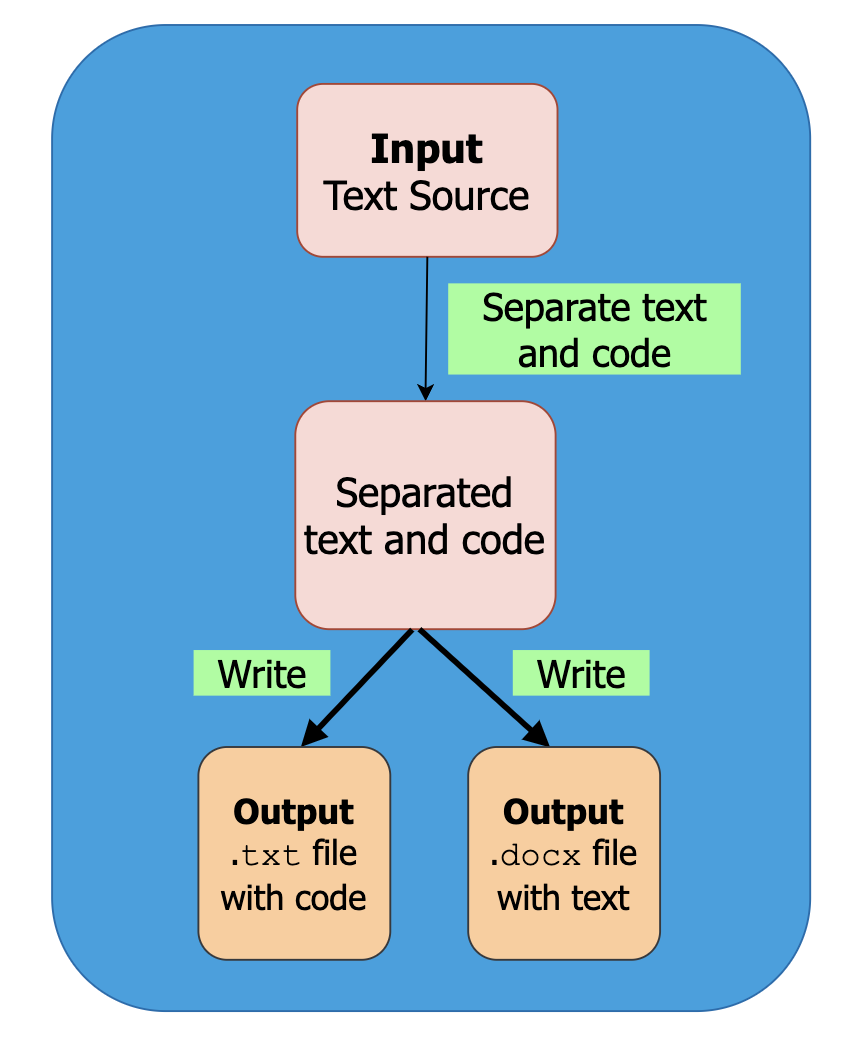
\includegraphics[width=0.6\textwidth]{figures/NB-high-arch.png}
    \caption{High-Level Architecture of Code-Text Separation Pipeline}
    \label{fig:high-level-arch}
\end{figure}


% change this cause it is not consistent with the design later need to make it so that the actual things like the tags and the text tags are in the boxes and the processes are on the arrows. 
The \textbf{high-level architecture} consists of the following:
\begin{enumerate}
    \item Get the contents of the text source
    % \item Parsing the response obtained from the HTTP libraries into Tags from the \texttt{tagsoup} library.
    % \item Separating the text from the code snippets using the descriptions of each Tag from the above Tags
    \item Separate the code snippets from the text.
    \item Writing the code snippets into a \texttt{.txt} file.
    \item Write the non-code textual content into a \texttt{.docx} file.
\end{enumerate}


\newpage 


\section{High-Level Design}


\begin{figure}[h]
    \centering
    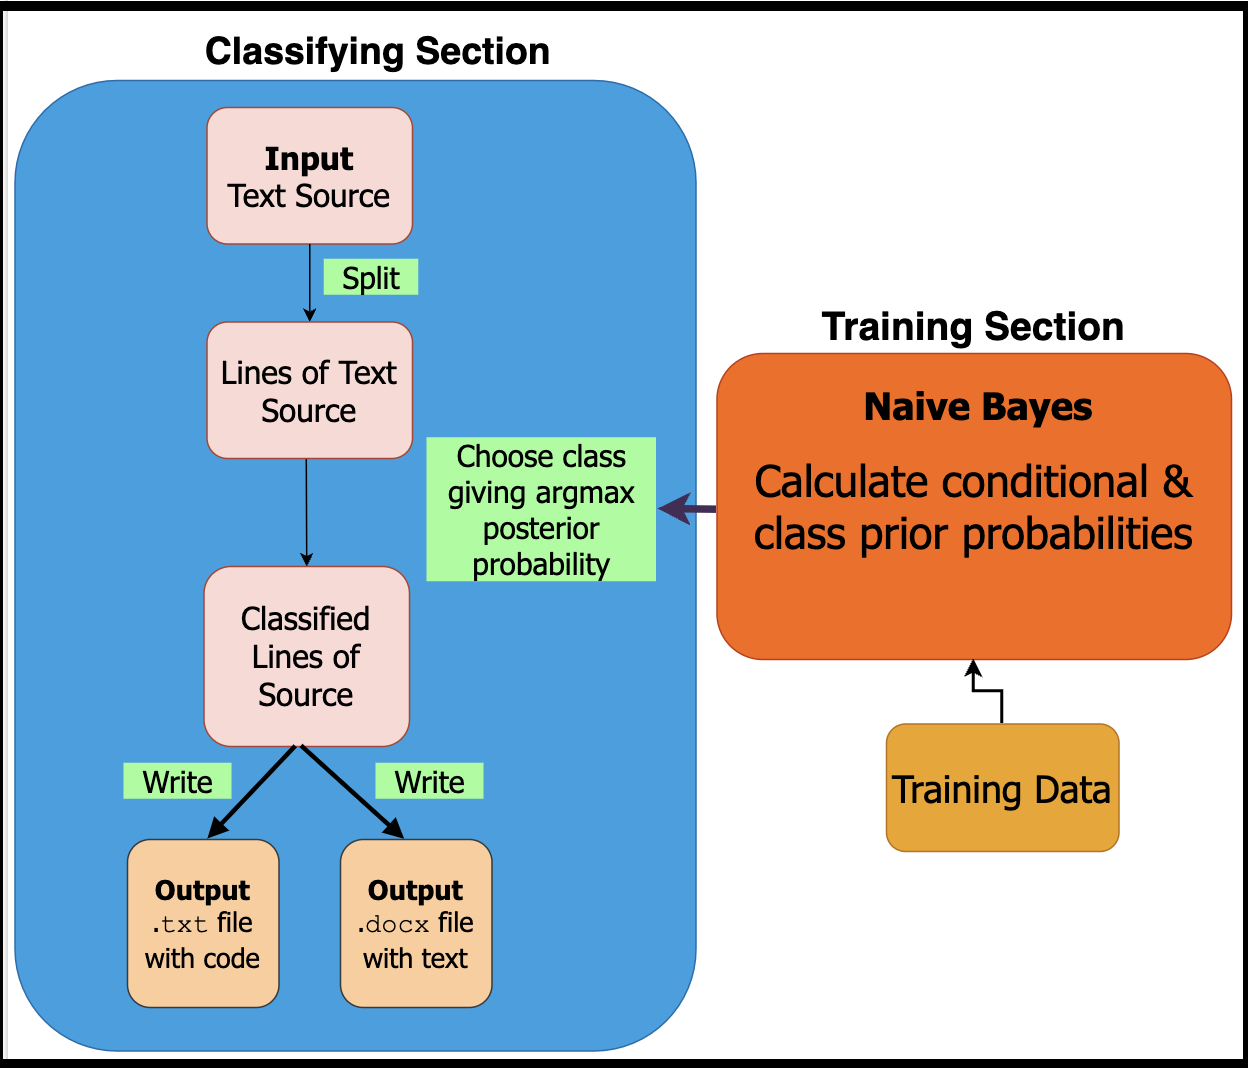
\includegraphics[width=1.0\textwidth]{figures/NB-high-design.png}
    \caption{High-Level Design of the Classifying Pipeline and Training Section}
    \label{fig:high-level-design}
\end{figure}

A more detailed description of the \textbf{high-level design} which implements the architecture broadly consists of two sections:
\begin{enumerate}
    \item \textbf{Training Section : }
    \begin{enumerate}
        \item Use natural language and source code training data already pre-classified in order to calculate the conditional probabilities and the class priors which make up the trained Naive Bayes Model.
    \end{enumerate}
    



    \item \textbf{Separation Pipeline Section : }
    \begin{enumerate}
        \item Split the given text source into lines which will be considered as separate "documents" by the trained classificaton model.
        \item Classify each different line as source code or natural language text depending on which class has the higher posterior probability given that line
        \item Write the lines classified as source code into a \texttt{.txt} file
        \item Write the lines classified as natural language text into a \texttt{.docx} file
        % \item Execute an HTTPS request for fetching the HTML contents of the web page
        % % \item Parsing the url into a request
        % % \item Executing the request with the TLS manager
        % \item Get the body i.e. the HTML content from the response received after executing the request
        % \item Parse the HTML into a list of Tags according to the \texttt{tagsoup} library
        % \item Separate the Tags corresponding to the code from the Tags corresponding to the textual content. By inspecting the HTML, we can see that the code snippets are within \texttt{<pre>} tags, so we need to separate everything enclosed within these tags from the rest of the HTML content. We also remove images. 
        % \item Insert delimiters between each different code snippet for formatting purposes. 
        % % \item Convert the list of Tag Strings corresponding to the code and to the text each back into an HTML-formatted string, which we then convert into a \texttt{pandoc} document as intermediate representation
        % % \item Convert the pandocs into another intermediate string-like format which can then be written into the respective \texttt{.docx} and \texttt{.txt} files
        % \item Convert the Tags back to HTML
        % \item Write the code snippets to the \ttt{.txt} file
        % \item Write the non-code textual content to the \ttt{.docx} file
    \end{enumerate}

\end{enumerate}

The lower level implementation details are mentioned in the implementations section. 

%  should i specify network stuff here?

% I don't think I should mention the evaluation section since that doesn't affect the system. That part should go into results and anyway not much to talk about over there







\chapter{Work Done: Implementation Details}
% this can give a broad overview of what the prototype can and cannot do. What the input and output of the prototype look like etc.


\section{File Structure}

% ?????????????????????????

\begin{verbatim}
scraper
|-- app
|   | -- Main.hs (main driver code)
|-- test
|   |-- Spec.hs (tests)
|-- src
|   |-- Lib.hs (implementation of functions)
|-- input
|   | -- lang_train.txt (training data)
|   | -- code_train.txt (training data)
|-- cases
|   | -- code_test{1-7}.txt
|   | -- lang_test{1-7}.txt
|-- output_files
|   | -- NB_code_class.txt (code snippets)
|   | -- NB_lang_class.docx (textual content)

\end{verbatim}




% in limitations can mention that need newline separated lines and we can't go beyond the granularity of a line since we did lines as documents based analysis



\section{Features and limitations}
% why mentioning this here?
The system mostly correctly identifies the code and text portions of the text source and writes them into the \texttt{.txt} and \texttt{.docx} files as per the requirements and specifications. While it doesn't meet the requirments to the fullest extent, some error will be unavoidable in such a lightweight yet generalizable approach. 

\subsubsection{Limitations}

\begin{enumerate}
    \item As mentioned, the system works on the granularity of a line and not a deeper token level granularity. Hence it can only attempt to classify whether a whole line is natural language or source code, without being able classify individual words or phrases within a line as being of a different class.
    \item Moreover, it cannot be used effectively in the case that the text source has data that is not separated by newlines, since each line is a document that needs to be classified here. However, these cases are relatively rare since most instances where code and natural language are found interspersed, there is some degree of organisation in terms of newline-separation.
    \item Since the system is relatively simplistic and unoptimized, along with the fact that it works on the Naive Bayes assumption of independence between features, it may not work well compared to other heavyweight methods in terms of accuracy. 
    \item Comments in the code written primarily in natural language will be classified as language and not code due to the nature of the classifier and the training data.
    \item It does not take into account the context in which a line has occurred, so the lines surrounding a particular line do not influence it's class, which is untrue in the real world.
\end{enumerate}

\section{Core Implementation Details}

Some important code and data details are shown.


% MAYBE ALSO REMOVE SOME OF THE EVALUATION STUFF CAUSE THE CODE GETTING TOO LONG    

%  NEED TO HAVE A SECTION ABOUT THE DETAILS OF THE TRAINING DATA CAUSE THAT IS OBVIOUSLY ESSENTIAL TO THE SYSTEM

\subsection{Main.hs}

\subsubsection{Training and Main Classification Pipeline}
In-line with the design, architecture and choice of tools as mentioned above, we first obtain the contents of the text source and split based on newlines. Training is done since we wish to keep the Naive Bayes classifier dynamic in terms of the words in accounts for. Since training for Naive Bayes is relatively cheap, this can be done without much additional cost, as we will encounter in the performance testing section.\\
\\ In the below code, we train the Naive Bayes Classifier, then predict the classes of every line of the text source and finally separate the text and the code into \ttt{.txt} and \ttt{.docx} files.

\begin{minted}[%
    breaklines,
    mathescape,
    linenos,
    numbersep=5pt,
    frame=single,
    numbersep=5pt,
    xleftmargin=0pt,
    ]{haskell}
    read_text_source <- readFile "input/sample.txt"
    let text_source = lines read_text_source -- newlines
    let lang_train = "input/lang_train.txt"
    let code_train = "input/code_train.txt"
    mydata <- Lib.readTraining lang_train code_train
    let lang_data = fst mydata
    let code_data = snd mydata
    let trainedModel = Lib.trainNaiveBayes lang_data code_data

    let final_classes = Lib.classifyNaiveBayes text_source trainedModel
    let mapping = zip text_source final_classes
    let code_class = [x | x <- mapping, snd x == 0]
    let lang_class = [x | x <- mapping, snd x == 1]
    writeFile "output_files/NB_code_class.txt" (unlines (map fst code_class))
    writeToDocx "output_files/NB_lang_class.docx" (unlines (map fst lang_class))
   \end{minted}
   
\subsection{Lib.hs}

\subsubsection{trainNaiveBayes}

This takes the natural language and source code training data and returns the prior probability of a word being a source code word, the conditional probabilities and the vocabulary based on the training data. The description of the helper functions is given later below. 

\begin{minted}[%
    breaklines,
    mathescape,
    linenos,
    numbersep=5pt,
    frame=single,
    numbersep=5pt,
    xleftmargin=0pt,
    ]{haskell}

-- NLA refers to the hmatrix library
trainNaiveBayes :: [String] -> [String] -> (( Double, ([Double] , [Double]) ), Vocabulary )
-- the strange output type is due to packaging various things together
trainNaiveBayes natural_data source_data = 
    let source_words = concat (getWords source_data) -- [String]
        natural_words = concat (getWords natural_data)
        unique_src_words = getUniqueWords source_words
        unique_natural_words = getUniqueWords natural_words
        vocab = unique_src_words ++ unique_natural_words

        xTrain_src = myVectorizer vocab (source_data)
        xTrain_lang = myVectorizer vocab (natural_data)

        sourceCodeMatrix = xTrain_src
        naturalLanguageMatrix = xTrain_lang

        -- NLA.Matrix Double -> [Int]
        sum_src_cols = sumCols sourceCodeMatrix
        sum_lang_cols = sumCols naturalLanguageMatrix

        src_len = length source_data
        natural_len = length natural_data

        xgivenY_src = calcXGivenY src_len sum_src_cols
        xgivenY_lang = calcXGivenY natural_len sum_lang_cols

        prob_src_prior = (int2Double src_len) / (int2Double src_len + fromIntegral natural_len)

    in ((prob_src_prior, (xgivenY_src,xgivenY_lang)), vocab )
    
    
\end{minted}





\subsubsection{classifyNaiveBayes}

It takes the lines of the text source that we have to classify, along with the output of the trained Naive Bayes Model. Due to the conditional probabilities being very small numbers, we work in the logspace to prevent issues due to numerical underflow, as is the case with most Naive Bayes implementations.\\ 
\begin{minted}[%
    breaklines,
    mathescape,
    linenos,
    numbersep=5pt,
    frame=single,
    numbersep=5pt,
    xleftmargin=0pt,
    ]{haskell}
   
       
-- NLA refers to the hmatrix library
classifyNaiveBayes :: [String] -> (( Double, ([Double] , [Double]) ), Vocabulary ) -> [Int]
classifyNaiveBayes test_data trainedModel =
    let vocab = snd trainedModel
        xTest = (NLA.toLists (myVectorizer vocab (test_data)))
        test_len = length xTest
        y = NLA.fromLists [(replicate (test_len) (int2Double 0))]

        -- [Double]
        xgivenY_src = fst (snd (fst trainedModel))
        xgivenY_lang = snd (snd (fst trainedModel))
        prob_src_prior = fst (fst trainedModel)

        log_src = map log xgivenY_src
        log_lang = map log xgivenY_lang

        log_matrix = NLA.tr (NLA.fromLists [log_src, log_lang])

        -- (head (DM.toLists log_matrix))) :: [Double,Double]

        -- matrix mult
        prob1 = (NLA.fromLists xTest) NLA.<> (log_matrix)

        -- (head (DM.toLists prob1))) :: [Double,Double]
        logp = log prob_src_prior
        log_not_p = log (1 - prob_src_prior)

        prob1_trans = NLA.toLists (NLA.tr prob1)

        prob2 = map (\x -> x + logp) (head prob1_trans)
        prob3 = map (\x -> x + log_not_p) (head (tail prob1_trans))

        combined = [prob2, prob3]
        combined_mat = NLA.tr (NLA.fromLists combined)
        
        final_probs = map (\x -> if (head x) > (head (tail x)) then 0 else 1) (NLA.toLists combined_mat)
    in final_probs       
\end{minted}


\subsubsection{Important Helpers}
\begin{enumerate}
    \item \ttt{myVectorizer : } Gives a matrix where each row corresponds to a document i.e. line and each column is a word in the vocabulary. So an entry $(i,j)$ represents the word count of word $j$ from the vocab in document $i$. If supplied empty lists then we return a dummy value due to constraints arising from the matrix library.
    \item \ttt{matrixRow : } It corresponds to one row in the above matrix. For each word in the vocabulary it gets the count of that word in the current document.
    \item \ttt{wordCounts : } For a document, creates a mapping between each word in the document and the count of that word in the document.
    \item \ttt{sumCols : } Finds the sum of every column in the matrix i.e. finds the total occurences of each word across all documents.
    \item \ttt{calcXGivenY : } For each word in the vocabulary, we sum the number of times it has appeared in source code documents. We divide by the total number of source code documents to get the probability of each word being in source code. We do a similar thing for natural language. We add small decimal numbers as a form of Laplace smoothing to avoid 0 probability in case of completely unseen words for the unseen data.
\end{enumerate}

\begin{minted}[%
    breaklines,
    mathescape,
    linenos,
    numbersep=5pt,
    frame=single,
    numbersep=5pt,
    xleftmargin=0pt,
    ]{haskell}
   
-- each row in matrix corresponds to a document and each column to a word in the vocabulary. So an entry (i,j) represents the word count of word j from the vocab in document i
myVectorizer :: Vocabulary -> [Document] -> NLA.Matrix Double
myVectorizer vocab docs
    | vocab == [] = NLA.fromLists [[int2Double 0]] -- sinceFromlists doesn't accept empty lists
    | docs == [] = NLA.fromLists [[int2Double 0]]
    | otherwise = NLA.fromLists [matrixRow vocab doc | doc <- docs]


-- takes a vocab i.e. list of strings. for each word in the vocab, look it up in the wordcount map of that document. If found then return the count, if not then 0 since the vocab word is not in this particular document. So this array of ints corresponds to one row in the vectorized matrix i.e. represents the word counts of all the words in the vocabulary in this document. 
matrixRow :: Vocabulary -> Document -> [Double]
matrixRow vocab doc = [fromMaybe (int2Double 0) (lookup vocab_word mywordcounts) | vocab_word <- vocab]
  where mywordcounts = wordCounts doc


-- for a document i.e. (string), create list of (string, int) pairs which maps each word with it's count in the document. create tuple for each word in the form of (word, 1) then map with the addition function in order to count
wordCounts :: Document -> [(String, Double)]
wordCounts doc = Data.Map.toList $ fromListWith (+) [(oneword, int2Double 1) | oneword <- words doc]



-- individual words
getWords :: [String] -> [[String]]
getWords [] = []
getWords (x:xs)
    | '\n' `elem` x && length x == 1 = ["NEWLINE"]:getWords(xs)
    -- | words x == [] = x:getWords(xs) -- here need to check if newline to do newline, otherwise spaces also getting included which makes it bad 
    | otherwise = (words (T.unpack . T.toLower . T.pack $ x)):getWords(xs)
    

getUniqueWords :: [String] -> [String]
-- get all unique strings from list of strings
getUniqueWords = foldl (\seen x -> if x `elem` seen then seen else seen ++ [x]) []

sumCols :: NLA.Matrix Double -> [Double]
sumCols matrix = map sum (NLA.toLists (NLA.tr matrix))

calcXGivenY :: Int -> [Double] -> [Double]
calcXGivenY mylen my_cols_sum =  map (\x -> x + 0.001 / int2Double (mylen) + 0.9 ) my_cols_sum

   \end{minted}




\subsubsection{Writers to files}
\texttt{writeToDocx} takes the text that has been classified as natural language and writes it into a \texttt{.docx} file after some formatting in order to massage the text into a Pandoc-friendly format due to the absence of functionality to read a plainText document or string.

\begin{minted}[%
 breaklines,
 mathescape,
 linenos,
 numbersep=5pt,
 frame=single,
 numbersep=5pt,
 xleftmargin=0pt,
 ]{haskell}
 writeToDocx :: String -> String -> IO ()
 writeToDocx filepath lang_class  = do
     pandoc_lang <- runIO $ readHtml def ( TextConv.convertText ("<p>" ++ lang_class ++ "</p>" :: String ) :: T.Text )
 
     case pandoc_lang of
         Right x -> do
             y <- runIO $ writeDocx def x
             case y of
                 Right direct_pan -> do
                     LBS.writeFile filepath direct_pan
 
                 Left err -> Prelude.putStrLn $ "Error with pandoc writeDocx: " ++ show err
 
         Left err -> Prelude.putStrLn $ "Error parsing pandoc for natural language " ++ show err
 
     putStrLn "Completed writing to docx"
\end{minted}


\subsubsection{Functions used for Evaluations with Test Cases}

\begin{minted}[%
    breaklines,
    mathescape,
    linenos,
    numbersep=5pt,
    frame=single,
    numbersep=5pt,
    xleftmargin=0pt,
    ]{haskell}
    evalTests :: (( Double, ([Double] , [Double]) ), Vocabulary ) -> [String] -> IO [(Double, Double, Double, Double)]
    evalTests _ [] = return []
    evalTests trainedModel (x:y:xs) = do
        lang_test <- readFile ("cases/" ++ x)
        src_test <- readFile ("cases/" ++ y)
        let test_data = (lines src_test) ++ (lines lang_test)
        let final_probs = Lib.classifyNaiveBayes test_data trainedModel
        let mapping = zip test_data final_probs
        let src_test_len = length (lines src_test)
        let lang_test_len = length (lines lang_test)
        let yTest = replicate src_test_len 0 ++ replicate lang_test_len 1
        let test_accuracy_mapping = zip yTest final_probs
        rest <- evalTests trainedModel xs
        -- precision_code, recall_code, precision_lang, recall_lang
        return $ (Lib.evaluateNaiveBayes test_accuracy_mapping):rest

    evaluateNaiveBayes :: [(Int, Int)] -> (Double, Double, Double, Double)
    evaluateNaiveBayes mydata = 
        let total_actual_lang = sum (map fst mydata)
            total_actual_code = (length mydata) - total_actual_lang
            code_correct = filter (== (0,0)) mydata
            lang_correct = filter (== (1,1)) mydata
            code_wrong  = filter (== (0,1)) mydata
            lang_wrong  = filter (== (1,0)) mydata
    
            num_code_correct = length code_correct
            num_lang_correct = length lang_correct
            num_code_wrong = length code_wrong
            num_lang_wrong = length lang_wrong
            precision_code = int2Double num_code_correct / (int2Double num_code_correct + int2Double num_lang_wrong)
            recall_code = int2Double num_code_correct / ((int2Double num_code_correct) + int2Double num_code_wrong)
            precision_lang = int2Double num_lang_correct / (int2Double num_lang_correct + int2Double num_code_wrong)
            recall_lang = int2Double num_lang_correct / ((int2Double num_lang_correct) + int2Double num_lang_wrong)
        in (precision_code, recall_code, precision_lang, recall_lang)
   \end{minted}
 
\section{Training Data}

Due to paucity of appropriate training data for this project with respect to scope and relevance, I curated my own small training dataset comprising of code and natural language that is typically seen accompanying the code. While there were datasets with source code and natural language, they were of a larger scale than I intended, and I also wanted to train the model on a smaller dataset to show that it can be lightweight not just with respect to time, but also training data required for good performance.\\ 
\\ While I covered some variety of programming languages, I deliberately excluded some popular paradigms like functional and database programming in order to observe the performance of the classifier on code that was unlike the code it had seen before.  I also skewed the training data in favour of the C programming language to see the relatively good results even on skewed training data. The statistics of the training data are given as follows, along with the sources where I took them from. The code was cleaned to remove comments and other non-code text.
%  BUT I DIDN'T INCLUDE VARIETY OF PROGRAMMING LANGUAGES

%  unskew this away from C

%  can put a table here which summarises the training data

% insert table here that has as headings the name of a programming language and the lines of code in the training dataset
\begin{table}[h]
    \centering
    \begin{tabular}{|c|c|c|}
        \hline
        \textbf{Programming Language} & \textbf{Lines of Code} & Source \\
        \hline
        C & 1171 & \href{https://github.com/karpathy/llm.c/blob/master/train_gpt2.c}{Andrej Karpathy's Github} \\
        \hline
        Python & 461 & \href{https://github.com/scikit-learn/scikit-learn/blob/main/sklearn/covariance/_robust_covariance.py}{Sklearn's Github} \\
        \hline
        Java & 201 & \href{https://github.com/jenkinsci/jenkins/tree/master}{Jenkins Github} \\
        \hline
    \end{tabular}
    \caption{Training Data Statistics (Code)}
    \label{tab:training-data}
\end{table}





\begin{table}[h]
    \centering
    \begin{tabular}{|c|c|c|}
        \hline
        \textbf{Description} & \textbf{Words and Lines} & Source \\
        \hline
            
        CS50 Lec1 & 780 and 37 & \href{https://cs50.harvard.edu/college/2023/spring/notes/1/}{CS50 Lecture 1} \\
        \hline
        CS50 Lec6 & 229 and 11 & \href{https://cs50.harvard.edu/x/2023/notes/6/}{CS50 Lecture 6} \\
        \hline
        Python 4 Everybody Text & 4910 and 589 & \href{https://www.py4e.com/code3/intro.txt}{Python 4 Everybody} \\
        \hline

    \end{tabular}
    \caption{Training Data Statistics (Language)}
    \label{tab:training-data}
\end{table}





\section{Challenges and Mitigations}

Initially, I started the project by separating the code and text based on their HTML tags for the midterm project evaluation, but after feedback from Professor I decided to make the project much more generalized to any given text source instead of just HTML content due to the fragile nature of a system based on the latter. \\ I decided to implement the Naive Bayes algorithm from scratch due to it's ease of interpretability, simplicity, lightweightedness and surprisingly strong results. A brief outline of some challenges and mitigations are as follows:
\begin{enumerate}
    \item Before deciding on implementing Naive Bayes from scratch, I thought about using various methods like Hidden Markov Models and Support Vector Machines to create an ensemble learning method to classify text and code. However, library support in Haskell for these was not of good quality, hence I decided to implement Naive Bayes on my own.
    %  mention how good performance?
    \item In the implementation of Naive Bayes, another hurdle I faced was the inefficiency of the default \ttt{matrix} library in doing calculations with extremely large and sparse matrices, which was restricting me to training and testing sets of very small sizes, albeit with considerably good performance. So I looked for more efficient libraries and found the \ttt{hmatrix} library, which sped up computations by a large extent. Earlier a training and classification that took 2.5 minutes overall, now happened in 2.5 seconds. 
    \item The paucity of appropriate training data was also an issue. The few datasets that were relevant to the project, such as those containing source code along with some form of natural language (usually in the form of code comments) were all restricted to one language and were also immense for a classifier implemented from scratch without optimisations. Hence, I curated my own modestly size source code and natural language training data based on manual searching online. The small size of the dataset also highlighted how the lightweight model was still performing relatively well. 
    \item The Haskell language was itself relatively challenging to get used to throughout the project due to it's difference from the imperative languages I am used to. But after learning lambda calculus and spending time with the language, it became easier to use and I could appreciate the elegance of functional programming more, even though I am still not as accustomed to this paradigm as I would like to be. 
\end{enumerate}




% maybe this can go after implementation details
\chapter{Work Done: Tooling and Testing}

\section {Tools and Languages}
% tech stack
% need to be clear on cabal stack and haskell and stuff


\subsection{Languages}

Only Haskell was used for the project as mentioned in the problem statement.

\subsection{Tools}

\begin{enumerate}
    \item The Glasgow Haskell Compiler (GHC) is used for compilation.
    \item \href{https://docs.haskellstack.org/en/stable/}{Stack} is used as the build tool. This manages installing project dependencies, building and running the project and testing the project.
    
    % say that hmatrix was used cause fastest
    \item \textbf{Notable Libraries}:
    \begin{enumerate}
        \item \textbf{hmatrix : } The fastest numerical linear algebra library that I could find in order to speed up the entire process, according to one benchmark \cite{matrixbench}. 
        %  CITE THIS!!!!!! cause which benchmark u talking abt
        \item \textbf{hUnit : } The basic Haskell unit testing library.
    \end{enumerate} 
\end{enumerate}






\section{Testing}
% test individual functions 
% for the midterm eval at the end if have time (need to) then can write one big test 

% \section{Tools to be used for Testing}



\subsection{Test Suite Outline}

\begin{enumerate}
    \item \textbf{Unit Testing : } The following functions were unit tested in the \ttt{Spec.hs} file
    \begin{enumerate}
        \item \ttt{myVectorizer}, \ttt{matrixRow}, \ttt{wordCounts}, \ttt{getWords}, \ttt{getUniqueWords} : Various sample inputs and expected outputs were provided and asserted to be equal. 

    \end{enumerate}

    \item \textbf{Performance Testing : } 
    % criterion and command line tools?
    \begin{enumerate}
        \item Test the time taken for the full system to execute from start to finish
        \item Test the memory consumption of the system
    \end{enumerate}
    \item \textbf{Functional Testing : } \\ Test whether the program meets the requirements by using sample input text sources and sample output files
\end{enumerate}






% \chapter{Plan for Completion}
% % will test. will do error handling. formal verification and validation stuff and maybe make more robust for other urls also idk. Getting better performance


% \begin{itemize}
%     \item Implement error handling gracefully wherever possible so that no unhandled errors can occur.
%     \item Implement the test suite
%     \item Attempt to make the scraper more generalized so that it can work with other websites and other HTML structures.
%     \item Document the code well
%     \item Explore methods of separating the code from the non-code textual content that are independent of HTML structure. Such methods were mentioned in the analysis and implementation of these methods will make the scraper more generalizable. 
% \end{itemize}


\chapter{Results and Discussions}


\section{Testing the Naive Bayes Classifier}

The classifier was run on various natural language and source code files and the results were collected. Metrics like precison and recall with respect to code and language were calculated. We found that even with the highly simplistic design and the strong Naive Bayes assumptions, the classifier could perform surprisingly well in classifying lines as code or natural language, subject to the limitations mentioned earlier.


% insert table here

\begin{table}[h]
    \centering
    \begin{tabular}{|c|c|}
        \hline
        \textbf{Case} & Code Details \\
        \hline
        Test 1 & \href{https://eli.thegreenplace.net/2018/type-erasure-and-reification/}{Supplied Web Page} containing C, Python, Java \\
        \hline
        Test 2 & Assembly Code from the \href{https://github.com/chrislgarry/Apollo-11/blob/master/Luminary099/AOSTASK_AND_AOSJOB.agc}{Apollo Guidance Computer} \\
        \hline
        Test 3 & SQL Code from \href{https://dev.to/tyzia/example-of-complex-sql-query-to-get-as-much-data-as-possible-from-database-9he}{this blog} \\
        \hline
        Test 4 & Haskell Code from \href{https://github.com/koalaman/shellcheck}{ShellCheck}\\
        \hline
        Test 5 & Mix of Python and C Code\\
        \hline
        Test 6 & Java Code\\
        \hline
        Test 7 & Python Code\\
        \hline
    \end{tabular}
    \caption{Test Case Details (Code)}
    \label{tab:results}
\end{table}
Details about the natural language test cases are not provided since difference in the data sources for natural language was found to not have much difference in accuracy.

\begin{table}[h]
    \centering
    \begin{tabular}{|c|c|c|c|c|}
        \hline
        \textbf{Test} & \textbf{Precision (Code)} & \textbf{Recall (Code)} & \textbf{Precision (Language)} & \textbf{Recall (Language)} \\
        \hline
        1 & 0.918 & 0.975 & 0.956 & 0.86 \\
        \hline
        2 & 0.997 & 1.0 & 1.0 & 0.889 \\
        \hline
        3 & 0.979 & 0.92 & 0.667 & 0.889 \\
        \hline
        4 & 0.967 & 0.93 & 0.474 & 0.667 \\
        \hline
        5 & 0.992 & 0.89 & 0.383 & 0.9 \\
        \hline
        6 & 0.978 & 0.986 & 0.882 & 0.833 \\
        \hline
        7 & 0.956 & 0.869 & 0.435 & 0.714 \\
        \hline
    \end{tabular}
    \caption{Test Case Results}
    \label{tab:results}
\end{table}

\subsection{Discussion}

As we can see in Table 10.2, we enjoy surprisingly good performance in a lot of cases. The precision and recall for the code is higher than that of natural language for most of the cases. The scores for natural language are mostly low, with only a few of the metrics going above the 80 \% mark while others are abysmal. Let's take a closer look at why some test cases have lower metrics. \\ 
\\ Consider the language precision of test case 5. This is low since the code contained many natural language comments that should have been classified as code, but were classified as natural language due to the nature of the classifier, thus lowering the precision. To properly classify such comments as code we either need to have the context of the surrounding lines or use a regular expression based approach that looks for comment patterns in various languages. The first approach increases the compute and complexity of the system, while the second approach is prone to errors and could classify some natural language as code instead.\\
\\ It is also important to note that the while classification accuracy is high, the format of the output files still leaves much to be desired in terms of the information that can be extracted from it, since it just comprises the code without any additional formattinng. However, in many cases, we have largelyn acheived the requirement of separating text and code snippets from a text source with relatively high accuracy.\\
\\ Lastly, these high rates of accuracy were acheived despite the training data not having some programming languages and being skewed in favour of a particular programming language. A possible explanation for this behaviour can be that a line in any programming languages, even extending to SQL and Assembly, have particular patterns in terms of numbers, special symbols and characters that make it easily differentiable from a natural language line. However, this is purely a hypothesis and needs rigorous testing and analysis.





\section{Software Testing Report}

\begin{enumerate}
    \item \textbf{Unit Testing : } All the unit tests passed successfully.
    \item \textbf{Performance Testing : }
    \begin{enumerate}
        \item With the command \ttt{stack run --profile -- +RTS -p} we can see the time and resource consumption on one particular run of the \ttt{stack run} command. Running it on the given text \href{https://eli.thegreenplace.net/2018/type-erasure-and-reification/}{source}, we see that it took \ttt{1.32} seconds to run and was allocated \ttt{5,774,171,368} bytes. \\ When it was given the entire text of Frankenstein comprising around 75,000 words and 1665 lines, it took \ttt{3.74} seconds to finish, which showcases it's relatively high speeds even considering training, due to the simplistic and linear nature of Naive Bayes.
        % For varying lengths of input the system took the following amounts of time to run
        % \item For varying lengths if input the system consumed the following amounts of resources
    \end{enumerate}

    \item \textbf{Functional Testing : } It meets the requirements that it needed to meet since it separates most of the code and natural language into separate files in many cases. But due to the limitations of the Naive Bayes classifier, it also has many erroneous cases which violate the requirments and specifications of having text and code separately. 
    
\end{enumerate}








%  in the results can have one example of some natural language or code that gets misclassified

%  graphs and stuff


%  pie charts and stuff


% tables and stuff 


\chapter{Conclusions}
%  should highlight contributions
%  lightweight text and code separation in functional programming language so it can be easily verified or smth
% it's also very interpretable and linear time complexity stuff

In this project, I implemented a lightweight classifier being able to perform considerably well in the task of classifying lines of text and code. While more heavy-weight models will definitely perform better due to added concepts like bi-grams, context and larger and better training data, the Naive Bayes system that we have used is highly simple and interpretable. This in conjunction with it's considerably good performance, albeit with many caveats, make it a useful tool to have for the text and code separation task. Using this classifier with other methods in a unified manner can lead to better results, which need to be further investigated. 


\chapter{Extensions and Future Work}

\begin{enumerate}
    \item The system can be extended to overcome the various shortcomings of the Naive Bayes classifier. Some of the more important things that would need addressing in the future in order to make a better separator would be context and a wider window so that the classifier can make a more informed decision.
    \item The newline requirement can be waived if a method to induce newlines can be found through semantic methods, which would make previously unstructured text now feasible for the Naive Bayes classifier. 
    \item Better formatting and extracting knowledge from the output of the classifier also should be worked on in order to retrieve more information from the text sources. 
    \item Find a way to write to the Word Document through pandoc without going through the readHTML function in order to preserve some formatting. 
\end{enumerate}

\begin{thebibliography}{9}

    \bibitem{bachemail}
    A. Bacchelli, M. D’Ambros, and M. Lanza, “Extracting source code from e-mails,” in Program Comprehension (ICPC), 2010 IEEE 18th International Conference on, June 2010, pp. 24–33.

    \bibitem{bachcontent}
    A. Bacchelli, T. Dal Sasso, M. D'Ambros and M. Lanza, "Content classification of development emails," 2012 34th International Conference on Software Engineering (ICSE), Zurich, Switzerland, 2012, pp. 375-385, doi: 10.1109/ICSE.2012.6227177

    \bibitem{chattter}
    Chatterjee, Preetha \& Gause, Benjamin \& Hedinger, Hunter \& Pollock, Lori. (2017). Extracting Code Segments and Their Descriptions from Research Articles. 10.1109/MSR.2017.10. 

    \bibitem{cerulohmm}
    L. Cerulo, M. Ceccarelli, M. Di Penta, and G. Canfora, “A hidden markov model to detect coded information islands in free text,” in Source Code Analysis and Manipulation (SCAM), 2013 IEEE 13th International Working Conference on, Sept 2013, pp. 157–166.

    \bibitem{matrixbench}
    \href{https://github.com/Magalame/fastest-matrices}{https://github.com/Magalame/fastest-matrices}

    \bibitem{juraf}
    D. Jurafsky and J. H. Martin. Speech and Language Processing: An Introduction to Natural Language Processing, Computational Linguistics and Speech Recognition. Prentice Hall, 2nd edition, 2009.

\end{thebibliography}



\end{document}